\section{Simulazioni modello di Ising 1D}

%-----------------------------------------%
%				Prima slide				  %
%	   Caratterizzazione metropolis   	  %
%-----------------------------------------%
\begin{frame}
    \frametitle{Caratterizzazione con metropolis}
    \framesubtitle{}

    \begin{columns}
        \begin{column}{0.33\textwidth}
            \begin{block}{Termalizzazione}

                \begin{itemize}[itemsep=0.5em, label=$\diamond$]
                    \item $t_{ter}$ maggiori per $T \simeq T_c$
                    \item $t_{ter}^{max}\,\simeq\,500$ sweeps
                \end{itemize}

                \vspace{0.5cm}

                \centering
                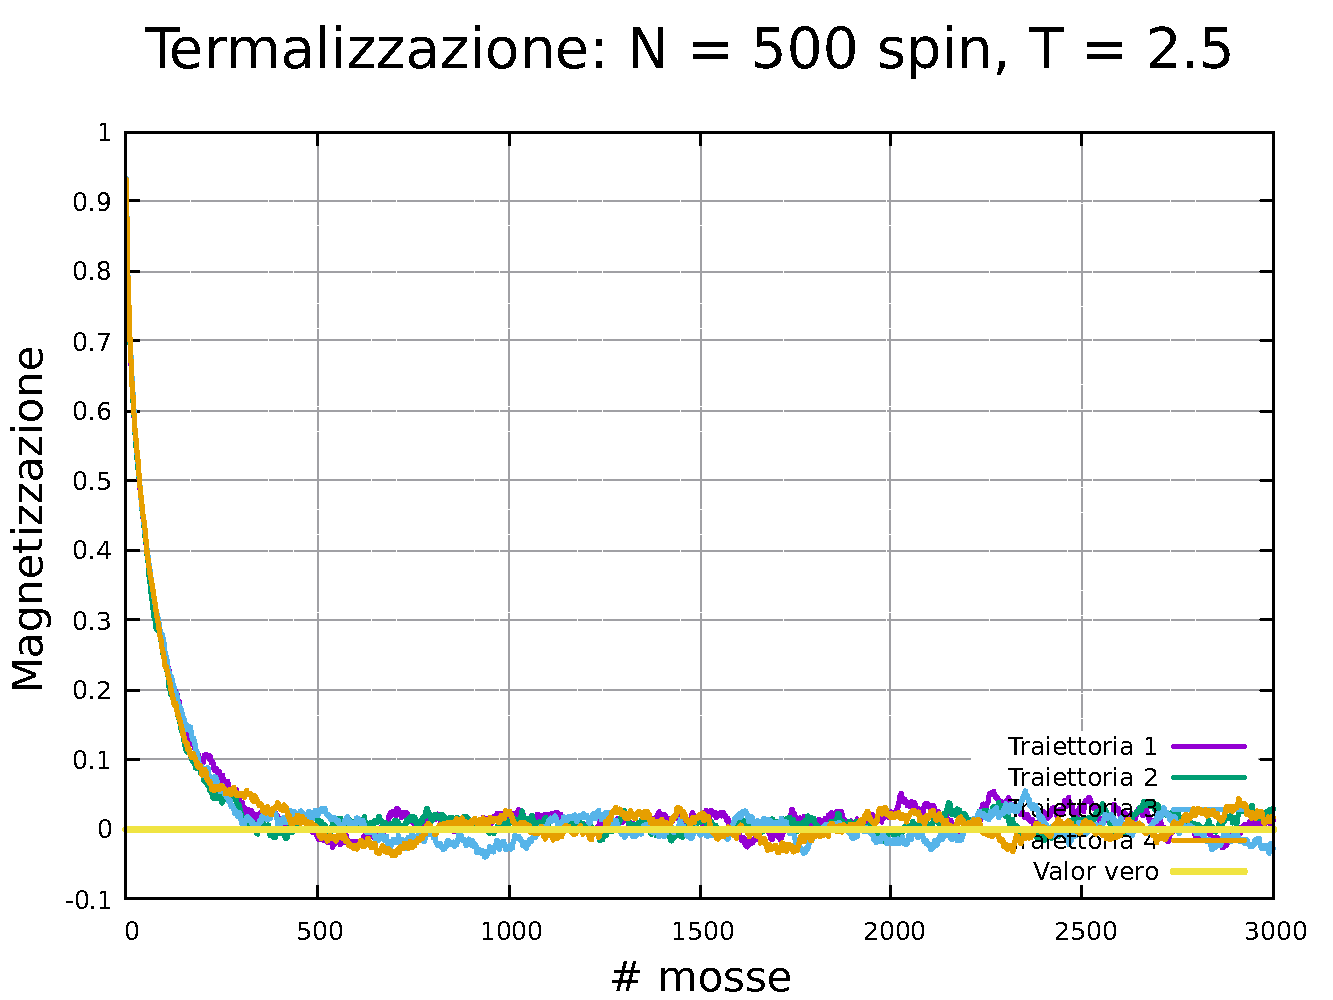
\includegraphics[width=\textwidth]{Immagini/simIsing2D/term_500_2.5.pdf}
            
            \end{block}
        \end{column}
    
        \begin{column}{0.33\textwidth}
            \begin{block}{Auto-correlazione}

                \begin{itemize}[itemsep=0.5em, label=$\diamond$]
                    \item $t_{c}$ maggiori per $T \simeq T_c$
                    \item $t_{c}^{max}\,\simeq\,400$ sweeps
                \end{itemize}

                \vspace{0.5cm}

                \centering
                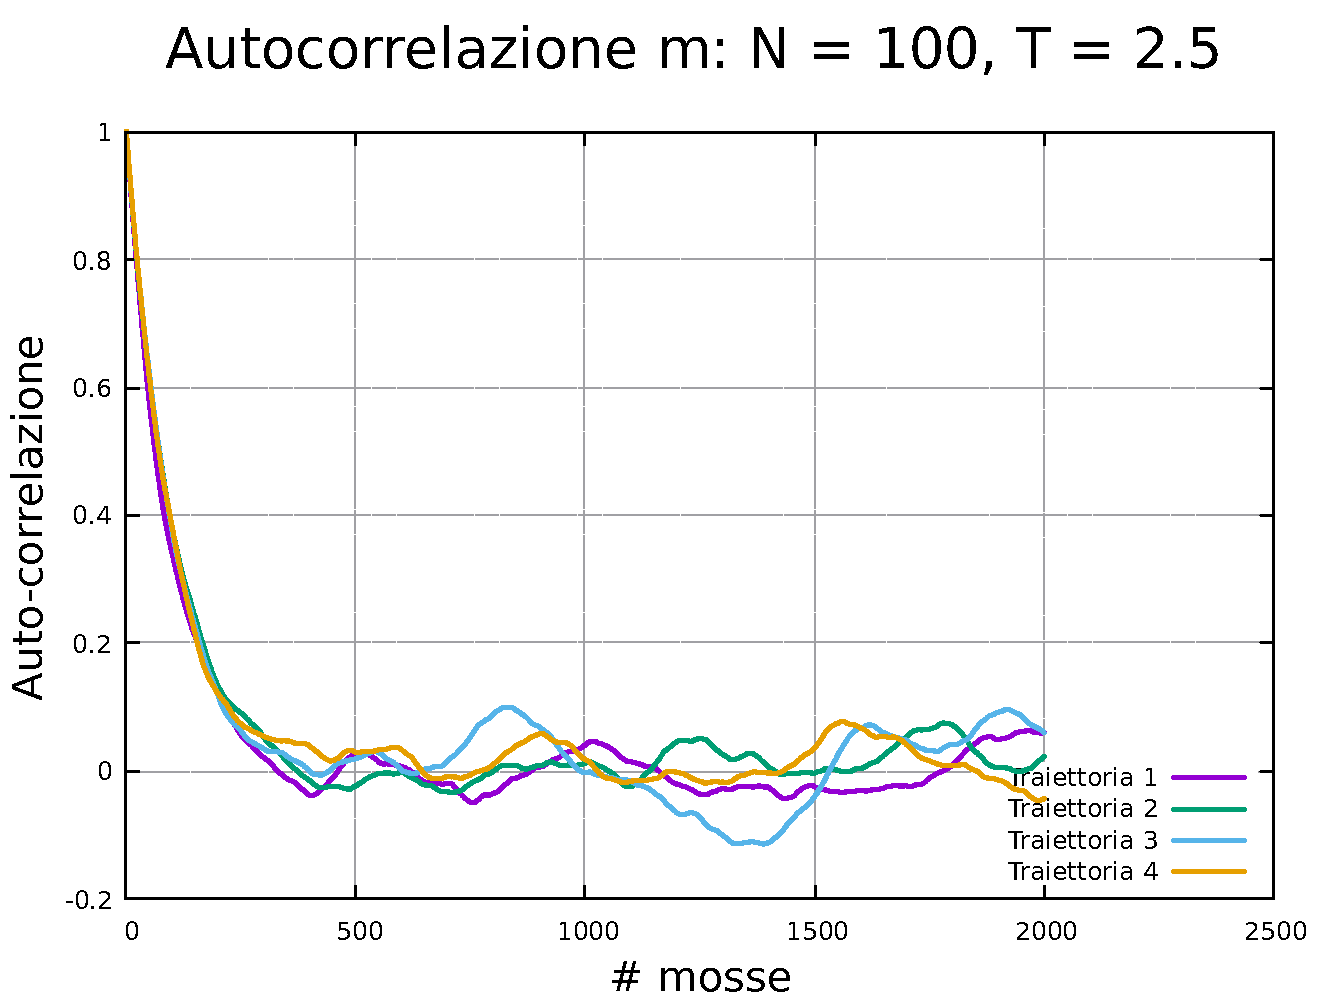
\includegraphics[width=\textwidth]{Immagini/simIsing2D/auto_100_2.5.pdf}
            
            \end{block}
        \end{column}

        \begin{column}{0.33\textwidth}
            \begin{block}{Blocchi}
                \begin{itemize}[itemsep=0.5em, label=$\diamond$]
                    \item $l_{blk}$ maggiori per $T \simeq T_c$
                    \item $l_{blk}^{max}\,\simeq\,1000$ sweeps
                \end{itemize}

                \vspace{0.5cm}

                \centering
                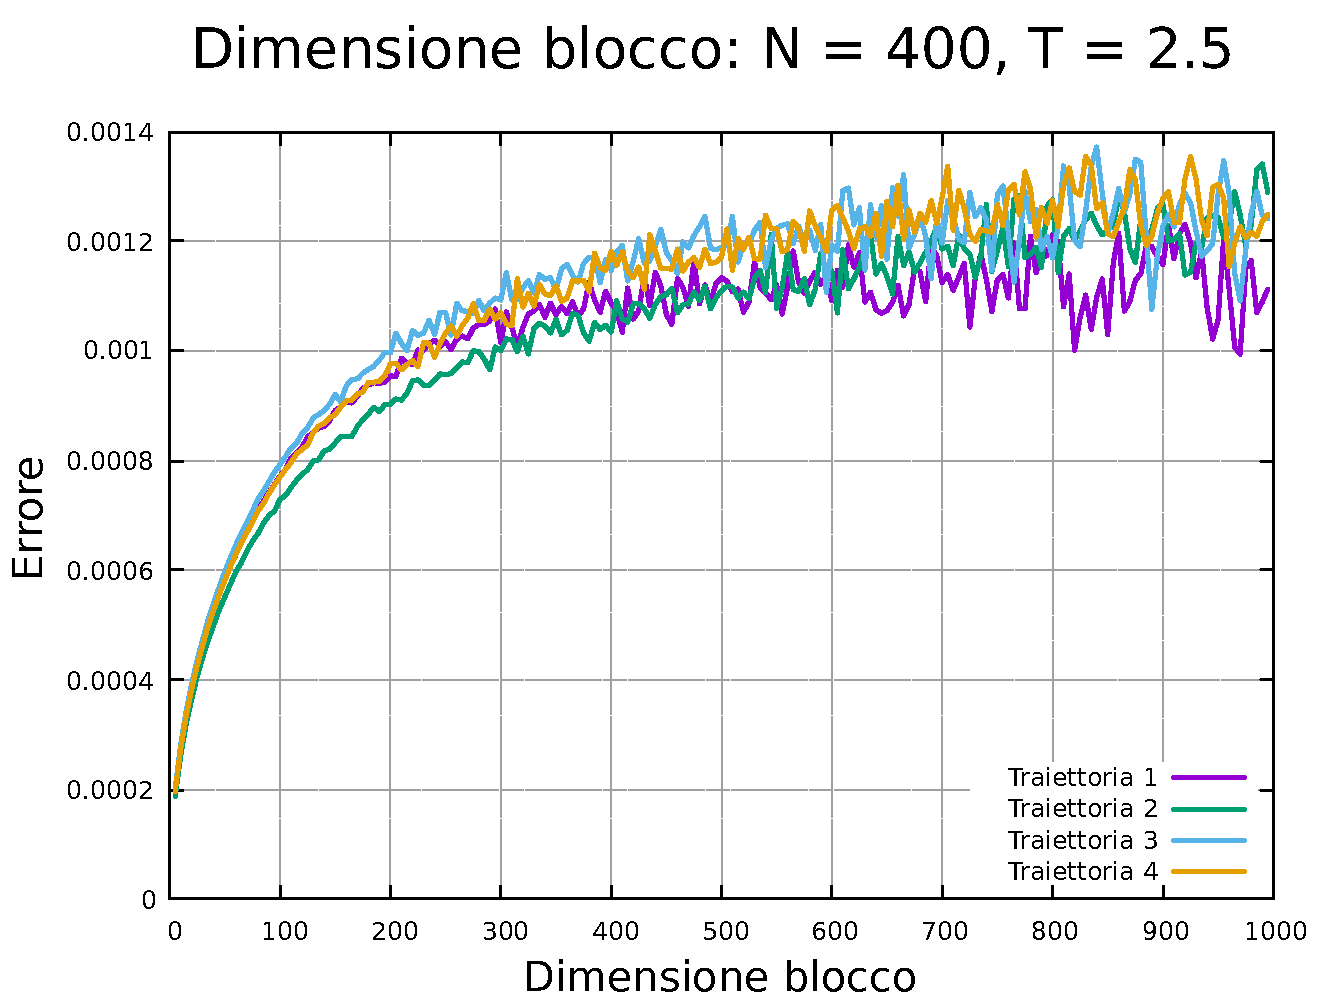
\includegraphics[width=\textwidth]{Immagini/simIsing2D/err_400_2.5.pdf}
            \end{block}        
        \end{column}
    \end{columns}
\end{frame}



%-----------------------------------------%
%		        Seconda slide	    	  %
%	      Caratterizzazione wolff   	  %
%-----------------------------------------%
\begin{frame}
    \frametitle{Caratterizzazione con Wolff}
    \framesubtitle{}

    \begin{columns}
        \begin{column}{0.33\textwidth}
            \begin{block}{Termalizzazione}
            
            \end{block}
        \end{column}
    
        \begin{column}{0.33\textwidth}
            \begin{block}{Auto-correlazione}

            \end{block}
        \end{column}

        \begin{column}{0.33\textwidth}
            \begin{block}{Blocchi}

            \end{block}        
        \end{column}
    \end{columns}
\end{frame}



%-----------------------------------------%
%			  Terza slide				  %
%	   Studio della magnetizzazione   	  %
%-----------------------------------------%
\begin{frame}
    \frametitle{Magnetizzazione}
    \framesubtitle{}

    \begin{columns}
        \begin{column}{0.6\textwidth}

            \centering
            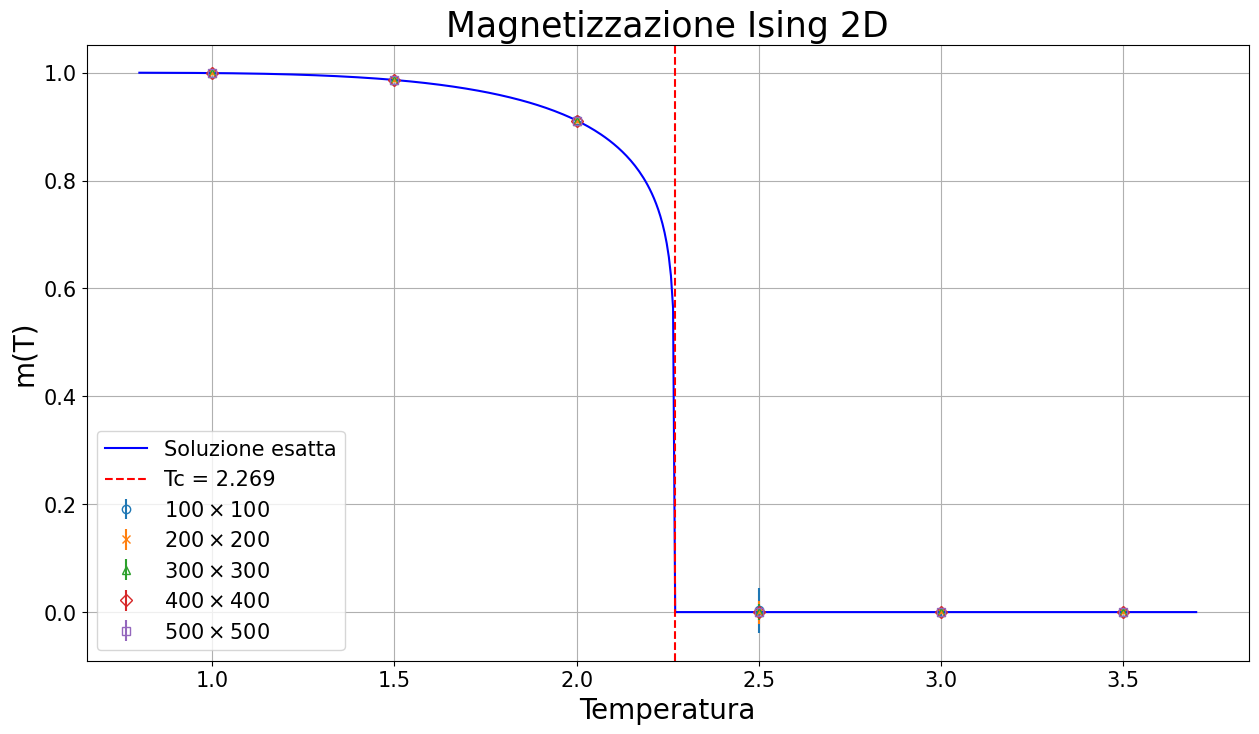
\includegraphics[width=\textwidth]{Immagini/simIsing2D/magn.png}

        \end{column}
    
        \begin{column}{0.4\textwidth}

                \begin{itemize}[itemsep=0.5em, label=$\diamond$]
                    \item Magnetizzazione spontanea per $T\,<\,T_c$
                    \item Transizione di fase a $T_c$
                \end{itemize}
            
        \end{column}
    \end{columns}

    \centering
    
\begin{tikzpicture}[thick, scale=1.2]
        \draw[->, line width=1mm] (0, 0) -- (10, 0);
        
        \node[below] at (0, 0) {Ferromagnetico};
        \node[below] at (10, 0) {Paramagnetico};
        
        \draw[fill=black] (5, 0) circle (2pt); 
        \node[above] at (5, 0) {$T_c$}; 
    \end{tikzpicture}

\end{frame}